\subsection{second best agent}

In this section, we describe how we trained our second-best agent. This agent initially imitates 
the rule-based agent and then seeks further improvement through deep Q-learning.

\begin{figure}[H]
    \centering
    
    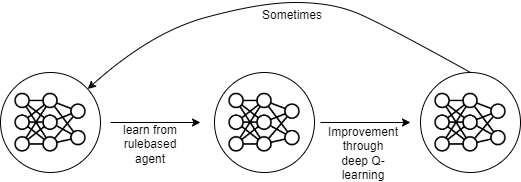
\includegraphics[width=\oneImgWidth]{images/training-strategy}%
    
    \captionadjust%
    \caption{\label{fig:training-strategy} Here is how we trained our second best model.
    }%
\end{figure}

Our initial idea was to develop an agent that starts by performing at the same level as the rule-based agent and then improves 
further through deep Q-learning. For this purpose, we had devised the following concept see \autoref{fig:training-strategy}.

Initially, our agent attempted to imitate the rule-based agent, as mentioned earlier. This was achieved through a classification approach. 
We collected the actions of the rule-based agent for each game state, and these actions served as the labels for the respective states. 
We gathered between 500,000 and 1,000,000 action-label pairs in this manner.
New data was added to the ReplayBuffer after each step until reaching the limit of 500,000 to 1,000,000 entries. 
After each round, specifically at the \verb|end_of_round| event, the following simplified function was executed to train our model.
Of course, the model was then also saved in an external file, which was achieved using Pickle.

\begin{lstlisting}[language=Python]
    ...
    
    def learn_rulebased_agent(model, labels, data, loss, opt, batch_size):
        train_ds = CTDataset(data, labels)
        train_dl = DataLoader(train_ds, batch_size=batch_size, shuffle=True)
        epoch_loss = 0

        ...

        for epoch in range(NUM_EPOCH):
            print("epoch %d / %d" % (epoch + 1, NUM_EPOCH))
            for i, (x, y) in enumerate(train_dl):
                opt.zero_grad()
                pred = model(x)
                loss_value = loss(pred, y) 
                loss_value.backward() 
                opt.step()
                epoch_loss += loss_value.item() 

            if epoch_loss <= 1e-5:
                break

            print(f"loss/epoch: {epoch_loss}")
            epoch_loss = 0      

    ...
    
\end{lstlisting}

First, we pass the model to the function that we want to train, followed by the labels, 
which represent the actions of the rule-based agent, and the data, which corresponds to the states. 
Then, we provide the loss function and optimizer, and finally, the batch size. We found that a batch size of 1024 worked well for us, 
especially as the model had more data to train on when the ReplayBuffer became fuller. We did experiment with other batch sizes,
but if the batch size was too small, it took a long time for the loss function to converge to 0 (which it didn't entirely reach).

We achieved good results when the \verb|num_epoch| was initially set at 2000, which we later increased to 5000 during training. 
Additionally, we sometimes had to remove older data from the ReplayBuffer to ensure that the model continuously learned from new games. 
It was also worthwhile to reduce the view box to 7x7 because it significantly reduced the number of possible states. 
After 4-5 days of training, our model became reasonably proficient at playing the game. While it couldn't perfectly mimic the rule-based agent, 
as the agent occasionally had to make random moves when there were no more items in its 7x7 view box, we still found the results quite satisfactory.

Afterward, we attempted to enhance the model using Q-learning. For this, we utilized the reward function from our best agent in the first project. 
Unfortunately, this approach didn't work well; the agent's performance deteriorated, and eventually, it struggled to play the game effectively. 
We saw improvement when we alternated training the model with the rule-based agent and then applied deep Q-learning see \autoref{fig:training-strategy}. 
However, even in this scenario, 
the results were significantly worse compared to when our model was solely imitating the rule-based agent.

In the end, we were unable to improve the agent using Q-learning beyond the level of our initial project, 
which we naturally submitted. We also considered reasons why we couldn't enhance the agent pre-trained with rule-based 
data using deep Q-learning. The main issue likely stems from optimizing the model with vastly different values when it imitates 
the rule-based agent compared to when it undergoes deep Q-learning. In the first case, the model is optimized with one-hot encoded 
actions of the rule-based agent, while in the latter case, it's optimized with the values of the reward function and the next states.